%\chapter{Further Installations}

\section{Generative Pre-Training 2 - X Large Model}

The `large' 774M model of GPT2 was ultimately released to the public. In addition, two other models were created: `x-large' had 1.5B parameters, and `xx-large,' had 8.3B parameters. The `x-large' was downloaded for testing.

Though tests from the previous sections worked on the `large' 774M model, subjectively the answers provided by the 1.5B model were better. The answers were stronger grammatically.

The 1.5B model was too large for a Raspberry Pi, using 12.3 Gig of RAM while it was running with inference. %The 1.5B model is experimented with on the development laptop computer.

As with the smaller model and the Raspberry Pi installation, no attempt was made to do transfer learning on the model. Instead the model was shown specific information during inference with which it was free to reply if it found the information appropriate.

%Additionally the model should be able to summarize articles from the internet and reply with that information when asked to do so. 

\label{chapter-gpt2-xl-intro}

\subsection{Context Experiment}

As before, the model was given details in sentence form that it could use as replies to questions when appropriate. The larger model worked better if all the sentences shown to it had the `Q:' and `A:' strings prepended to them. 

In each example, the information the model chose from was presented in sentence pairs. Though these sentences looked much like source/target pairs from our movie corpus, they were totally unrelated.

An example might be the presentation of its own name to the model. In the smaller GPT2 model, the model was shown the single sentence `My name is Jane.' In the larger GPT2 model's code, the model was shown two sentences. One was `Q: What is your name?' and the other, following it directly, was `A: My name is Jane.' These conventions were followed for time of day, the model's location, and the model's occupation.

These questions can be answered without any memory of the last question.

\subsection{History Experiment}

All input and output was concatenated and included with each question. This had little effect in the smaller GPT2 experiment, but the history questions were helpful with the larger models. Consider the questions below.
\begin{verbatim}
> Do you like the color red?
I like the color red.
> What is your favorite color?
Red.
\end{verbatim}
This was the same text excerpt as from the small GPT2 model in Section \ref{install-gpt2-history}. The `favorite color' example continued to work on the larger GPT2 model. Again, as in the small model, the chatbot was using the history in the conversation. 

Even though the history was consulted before answers are formulated, the output of the model was not always predictable. %This has something to do with the `temperature' setting of the model. The output is sometimes more fanciful.


\subsection{Artificial Intelligence Markup Language Experiment}

%We want to be able to tell the model exactly how to answer a given question if we have a particular need. 
The GPT2 models remembered the user's name very badly. %We would like to dictate how the model handles that situation. 
Artificial Intelligence Markup Language was used to improve this. 

AIML is actually poorly suited for handling this task. In AIML every question and response must be coded as a separate rule. For the question `How are you?' and answer `I am fine,' the AIML kernel will only answer with the programmed response if the input is an exact match. If the questions are `How are you doing?' or `How do you feel?' the kernel does not have any answers. %The two or three questions are phrased differently but can be answered with the same text.

The GPT2 chatbot is different. Groups of questions have the same answer. Sometimes the answer could even be `I don't know.' The chatbot could answer `I don't know' or `I am fine' to  `How are you,'  `How are you doing?' and `How do you feel?' These questions can be phrased differently with the same answer.

To use AIML for this task questions and answers were coded in pairs for all possible phrasings of a question.

%We have to count the number of AIML rules that we are coding and compare it to the number of English sentences that the GPT2 chatbot can answer. We have to make sure that the number of chatbot answers is much higher. As it stands the number of GPT2 chatbot answers dwarf the AIML rules.

%We prefer the answers provided by the generative chatbot over those provided by an AIML file. We want to maximize the amount of time that the overall model answers using the Transformer that is internal to the chatbot, and minimize the use of AIML and the AIML kernel. We set a criteria for ourselves. If the generative chatbot is handling most of the questions and answers then we can proceed. If the AIML question/answering set is larger than the number of questions that the chatbot can answer, then the AIML should be avoided. 

Two situations with AIML files are below.

\subsection{User Name Experiment}
%The name of the user is our first example of AIML coding. This example is easy. 
User name is the first example. Using `*' as a wildcard, there are a few ways to say ones name. One way is `My name is *.' Another variant is `* is my name'. %That's as many ways to say it as there are.

Each question is answerable with a phrase like `Hello *.' The asterisk is still a wildcard for the memorized name. An AIML file can handle this sort of question very easily. %We write an AIML file with these questions. We depend on the AIML to remember the name from the wildcard. 

Another question in this scenario is `What is my name?' In AIML there are very few ways to phrase this question. %With this question also there are very few ways to phrase the AIML. %Here we are referring to the name recorded in the previous AIML question as discussed above. 

During a typical chatbot run the AIML kernel is shown all user input.% to the AIML kernel. 

When the kernel does not match anything there is no output. When there is a match, AIML output is shown to the chatbot as the context for that input. 
%Input from the user is concatenated with the context text, the answer from the AIML kernel. 
The chatbot is then left to choose what to answer from the question and the context. 
%Usually the answer makes sense.

The question and the chatbot answer are both added to the history. 
This history is retained. 
%what the user enters and the chatbot's answer are kept by the chatbot so that the chatbot can keep track of answers over time. 
Sometimes, though, keeping sentences that refer to user names confuses the bot's answers.% In other cases the bot keeps track of answers that are generated in the AIML/chatbot hybrid process.

Even when the answer is sensible the model's answer is not always correct, but without the AIML the model always answers all name questions with it's name. 

%We suspect if the model was much larger that it would have less trouble with this kind of example.

\subsubsection{Usage Example}

The user might say `Hello, my name is John.' The bot might reply `Hello.' The user might then say `What is your name?' The bot should reply `My name is Jane.'

Then the user might say `What is my name?' The bot should reply `John.'

%In practice the bot will reply with `Jane' most of the time. % without the AIML augmentation. 
With the smaller GPT2 model the reply to this is often `Jane.' %even with the AIML kernel. 
With the larger GPT2 model the bot tends to answer what the AIML suggests. In this case the answer would be `John.'

\subsection{Internet Search Experiment}
The model is asked a question and an article is downloaded from the Internet, and summarized. % to answer the question.
%We want to be able to search the internet for an article, download that article, and summarize parts of the article as answers to questions asked of the model. 

This is leveraging of the token size of the input to the model. It's usually very large. It can be 1024 tokens.

The AIML required is minimal but larger than the AIML for the `user name' problem. The goal is to detect, first, when the user wants to talk about an Internet page, and second, detect when they are done.

The first case, when the user wants to talk about an Internet page, is associated with utterances like `Tell me about *' and `I want to talk about *.' The asterisk is a wildcard for what the user is interested in. There can be other phrases that imply the user's intention. In these cases, the text from the wildcard in the invocation is saved.

The second case, when the user is done with the Internet page and wants to return to normal operation, is associated with utterances like `Ok thanks' and `That's enough.' 
%These two phrases can be checked for when the bot is in `Internet-Search' mode. 
There could be other phrases that cause the same operation in the AIML code.

When the AIML detects one of these signals, the program goes into a special mode of operation. The first, or `find' signal, causes operation of an Internet browser. The web search uses the text from the invocation of the `find' command. The browser yields results as they would be found using a Google search engine. The first 20 results are kept and the URL for the highest ranking Wikipedia page is retained. It is loaded and the `body' tag is scanned for `paragraph' type content. This information replaces the context input. 

After that, the context is retained while the chatbot answers any questions that the user might have. The GPT2 model has some facility with this, while the larger GPT2 model is more adept.

Later, when the AIML detects the second, `restore' signal, the program switches back from special operation to normal operation. Web page contents are removed and the context is restored. % as it was during regular chatbot use. 
%There is a part that has the history of the last few questions and answers, and there is a part that has the bot name, occupation, and the current time.

As the chatbot answers questions, the content of the conversation is stored as `history.' % of the context text, as it is used in the regular chatbot mode. 
This is a record of the chatbot operation even when it is answering questions about a web page. %that it has searched for. 
Because of size limitations, the history is not included in the chatbot input when it is answering questions about a web page. %, but a record is kept of `q' and `a' and the bot can refer to them later.

%Again, because of size restrictions there is no regular context information shown to the chatbot while it is answering questions about a web page. 

After the `restore' signal, the chatbot sees only the regular context and none of the web page material. The regular input size for all models is 1024 tokens. %and it is more than 1000 for the larger models. 
Though this would appear to be a large space for text, it is common for Wikipedia articles to be clipped so that the user's question can be inserted at the end.

\subsubsection{Usage Example}

This example uses the musical group `The Beatles.' The user's question is `Tell me about the Beatles.'

The chatbot takes seconds to download an article from Wikipedia. Ultimately it answers `The Beatles were an English rock band formed in Liverpool in 1960.'

The user asks `How many members were in the band?'

The 774M chatbot answers, `The Beatles were originally formed by John Lennon and Paul McCartney in Liverpool.' This is not the correct answer. This may be because, after clipping, that information does not exist in the context section. The user may ask other questions. %Some may be answered correctly.

To this question, the x-large model answers `There were four members in the band.' This is correct.

When the user asks `How many members were in the band?' the model seems to be able to answer with the specific band. % that you are referring to.

To end the Q/A session the user says `OK' or `OK thanks.' Though the web page for the `Beatles' would no longer be available to the chatbot, it could still answer `Beatles'  questions. The user could ask `What are the Beatles?' The answer might be, `The Beatles were an English rock band formed in Liverpool in 1960,' even though the Wikipedia page is not available to the bot.

\label{chapter-xlarge}

\section{Generative Pre-Training 2 - Jetson Nano}

\label{chapter-nano}
The Jetson Nano is a small single board computer that has a NVIDIA GPU. %It has 4 Gigabytes of ram and runs on the aarch64 platform.

 %The Nano uses an NVIDIA GPU.
Initial tests showed a 117M GPT2 model could answer a basic question in two to three seconds. Previously a Raspberry Pi computer took thirteen or fourteen seconds. On the host laptop, where development was done, the 117M model still outperformed the Nano, responding to a general question in one second.
%It was used as a platform for the GPT2 117M parameter model.

The smaller 117M parameter model was not used for the Wikipedia searches that were attempted in Section \ref{chapter-gpt2-xl-intro}. It was used for the same basic chatbot task tested on the Raspberry Pi platforms.

%Some details from this experiment are identical to Section \ref{install-gpt2-chatbot} or Section \ref{install-gpt2-smart} where the 117M model is installed on a Raspberry Pi.

The Nano that the GPT2 model was installed on was outfitted with a speaker, a microphone, and a WiFi dongle. Pytorch for the Nano was installed from a community web site where version 1.5 or 1.6 was already cross-compiled for the aarch64 environment. 

Response time with the Nano was five seconds. Response time on the Raspberry Pi for the 117M model was 14 seconds. (See the discussion of `Reply Time' in Section \ref{setup-reply-time}.)

\begin{figure}[H]
	\begin{center}
		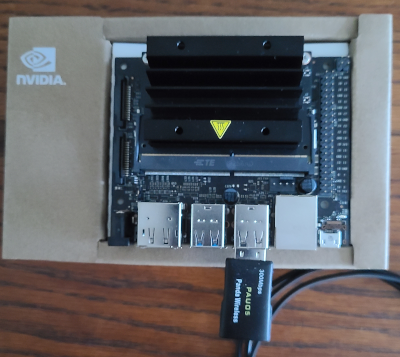
\includegraphics[scale=0.9]{diagram-jetson-nano-02}
		
		
	\end{center}
	\caption[Jetson Nano]{Jetson Nano without case.}
	
	
\end{figure}